\chapter{Mediciones y Resultados}
En el presente capítulo se resumirán las mediciones realizadas y los resultados obtenidos luego del desarrollo de los biosensores. Se dividirá en tres procedimientos diferenciados por el tipo de caracterización: eléctrica, dimensional y electroquímica.

\section{Caracterización eléctrica}
Se realizaron las mediciones de resistencia a cuatro puntas obteniendo los siguientes resultados:

$\bullet$ Entre dos pads de carbono: \textbf{2,2 k$\Omega$}.

$\bullet$ Mismos pads de carbono con una capa de tinta de nanopartículas de oro curado: \textbf{1,15 k$\Omega$}.

$\bullet$ Mismos pads de carbono con dos capas de tinta de nanopartículas de oro curado: \textbf{500 $\Omega$}.

Dada la deposición de la capa de tinta de oro sobre el carbono, se forma un paralelo entre los dos elementos. Utilizando la ecuación de resistencias en paralelo (\ref{ecuacion1}) puede calcularse la resistencia que posee la impresión de una y dos capas curadas de nanopartículas de oro.

\begin{equation}\label{ecuacion1}
R_{1//2}=\frac{R_{1} \times R_{2}}{R_{1}+R_{2}}
\end{equation}

De esta forma se obtienen los siguientes valores:

$\bullet$ Una capa de nanopartículas de oro curado: \textbf{2,4 k$\Omega$}.

$\bullet$ Dos capas de nanopartículas de oro curado: \textbf{0,65 $\Omega$}.


Asumiendo que las capas de Oro son impresiones de películas delgadas se utiliza la ecuación (\ref{ecuacion2}) para obtener la resistividad del material.

\begin{equation}\label{ecuacion2}
\rho_{Bulk}=\frac{R \times w \times t}{L}
\end{equation}

siendo $\rho$\textsubscript{Bulk} la resistividad, $R$ la resistencia, $w$ el ancho, $t$ el espesor y $L$ el largo del material. En este caso, la vía de nanopartículas de oro. El ancho del diseño es de 0,04 cm, el espesor promedio para dos capas 0,00055 cm (obtenido mediante perfilómetro) y el largo 1,05 cm dando los siguientes resultados:

$\bullet$ Una capa de tinta de nanopartículas de oro curado (asumiendo la mitad del espesor): \textbf{0,025 $\Omega$ $\times$ cm}

$\bullet$ Dos capas de tinta de nanopartículas de oro curado: \textbf{0,0000136 $\Omega$ $\times$ cm o 13,6 $\mu\Omega$ $\times$ cm}


Según la tabla de resistividad de los materiales, el oro puro posee una resistividad de \textbf{2,35 $\mu\Omega$ $\times$ cm} \cite{Resistividad}.

\section{Caracterización dimensional}
Luego de medir ópticamente los ocho electrodos de un cartucho, se promedió el diámetro en \textbf{993 $\mu$m} y las separaciones entre elementos de la celda electroquímica en \textbf{390 $\mu$m}.

En la tabla de la figura~\ref{fig:Figura_tabla_rugosidades} se muestran los resultados de las rugosidades obtenidas.

\begin{figure}[H]
  \centering
    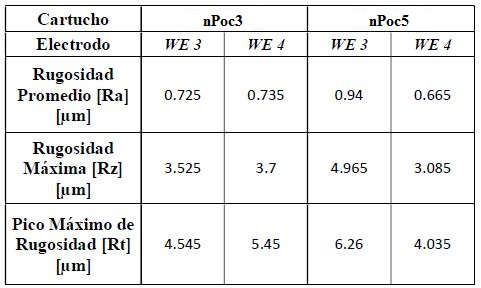
\includegraphics[width=0.6\textwidth]{Figuras/Figura_tabla_rugosidades}
  \caption{Valores de rugosidad obtenidos para dos \emph{WE} de dos biosensores (nPoc3 y nPoc5).}
  \label{fig:Figura_tabla_rugosidades}
\end{figure}

Se midieron los espesores de los mismos \emph{WE} sobre los mismos biosensores. Para poder obtener el espesor estimado de las 2 capas impresas con la tinta de nanopartículas de oro, se midió el espesor sobre un electrodo de carbono puro.

En la tabla de la figura~\ref{fig:Figura_tabla_espesores} se muestran los valores obtenidos de los espesores.

\begin{figure}[H]
  \centering
    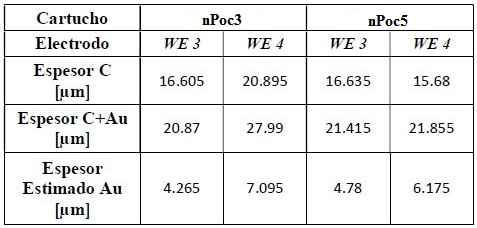
\includegraphics[width=0.6\textwidth]{Figuras/Figura_tabla_espesores}
  \caption{Valores de espesores obtenidos para dos \emph{WE} de dos biosensores (nPoc3 y nPoc5).}
  \label{fig:Figura_tabla_espesores}
\end{figure}

Las tablas fueron extraídas del informe realizado en el Centro de Física y Metrología del Instituto Nacional de Tecnología Industrial \cite{caracdimen}.
\newpage 
\section{Caracterización electroquímica}
La primera voltametría cíclica se realizó con un electrodo de oro puro depositado sobre silicio mediante un proceso de \textit{Sputtering}. Se obtuvo la respuesta para las sondas electroquímicas ferro y ferricianuro sobre un electrodo de oro depositado por \textit{sputtering}(Figura ~\ref{fig:Figura_EQ_Oro_Sputtering_1mm}), la cual se usará como referencia para comparar con los electrodos impresos con tinta de nanopartículas de oro mediante el proceso de impresión \textit{Inkjet}.

\begin{figure}[H]
  \centering
    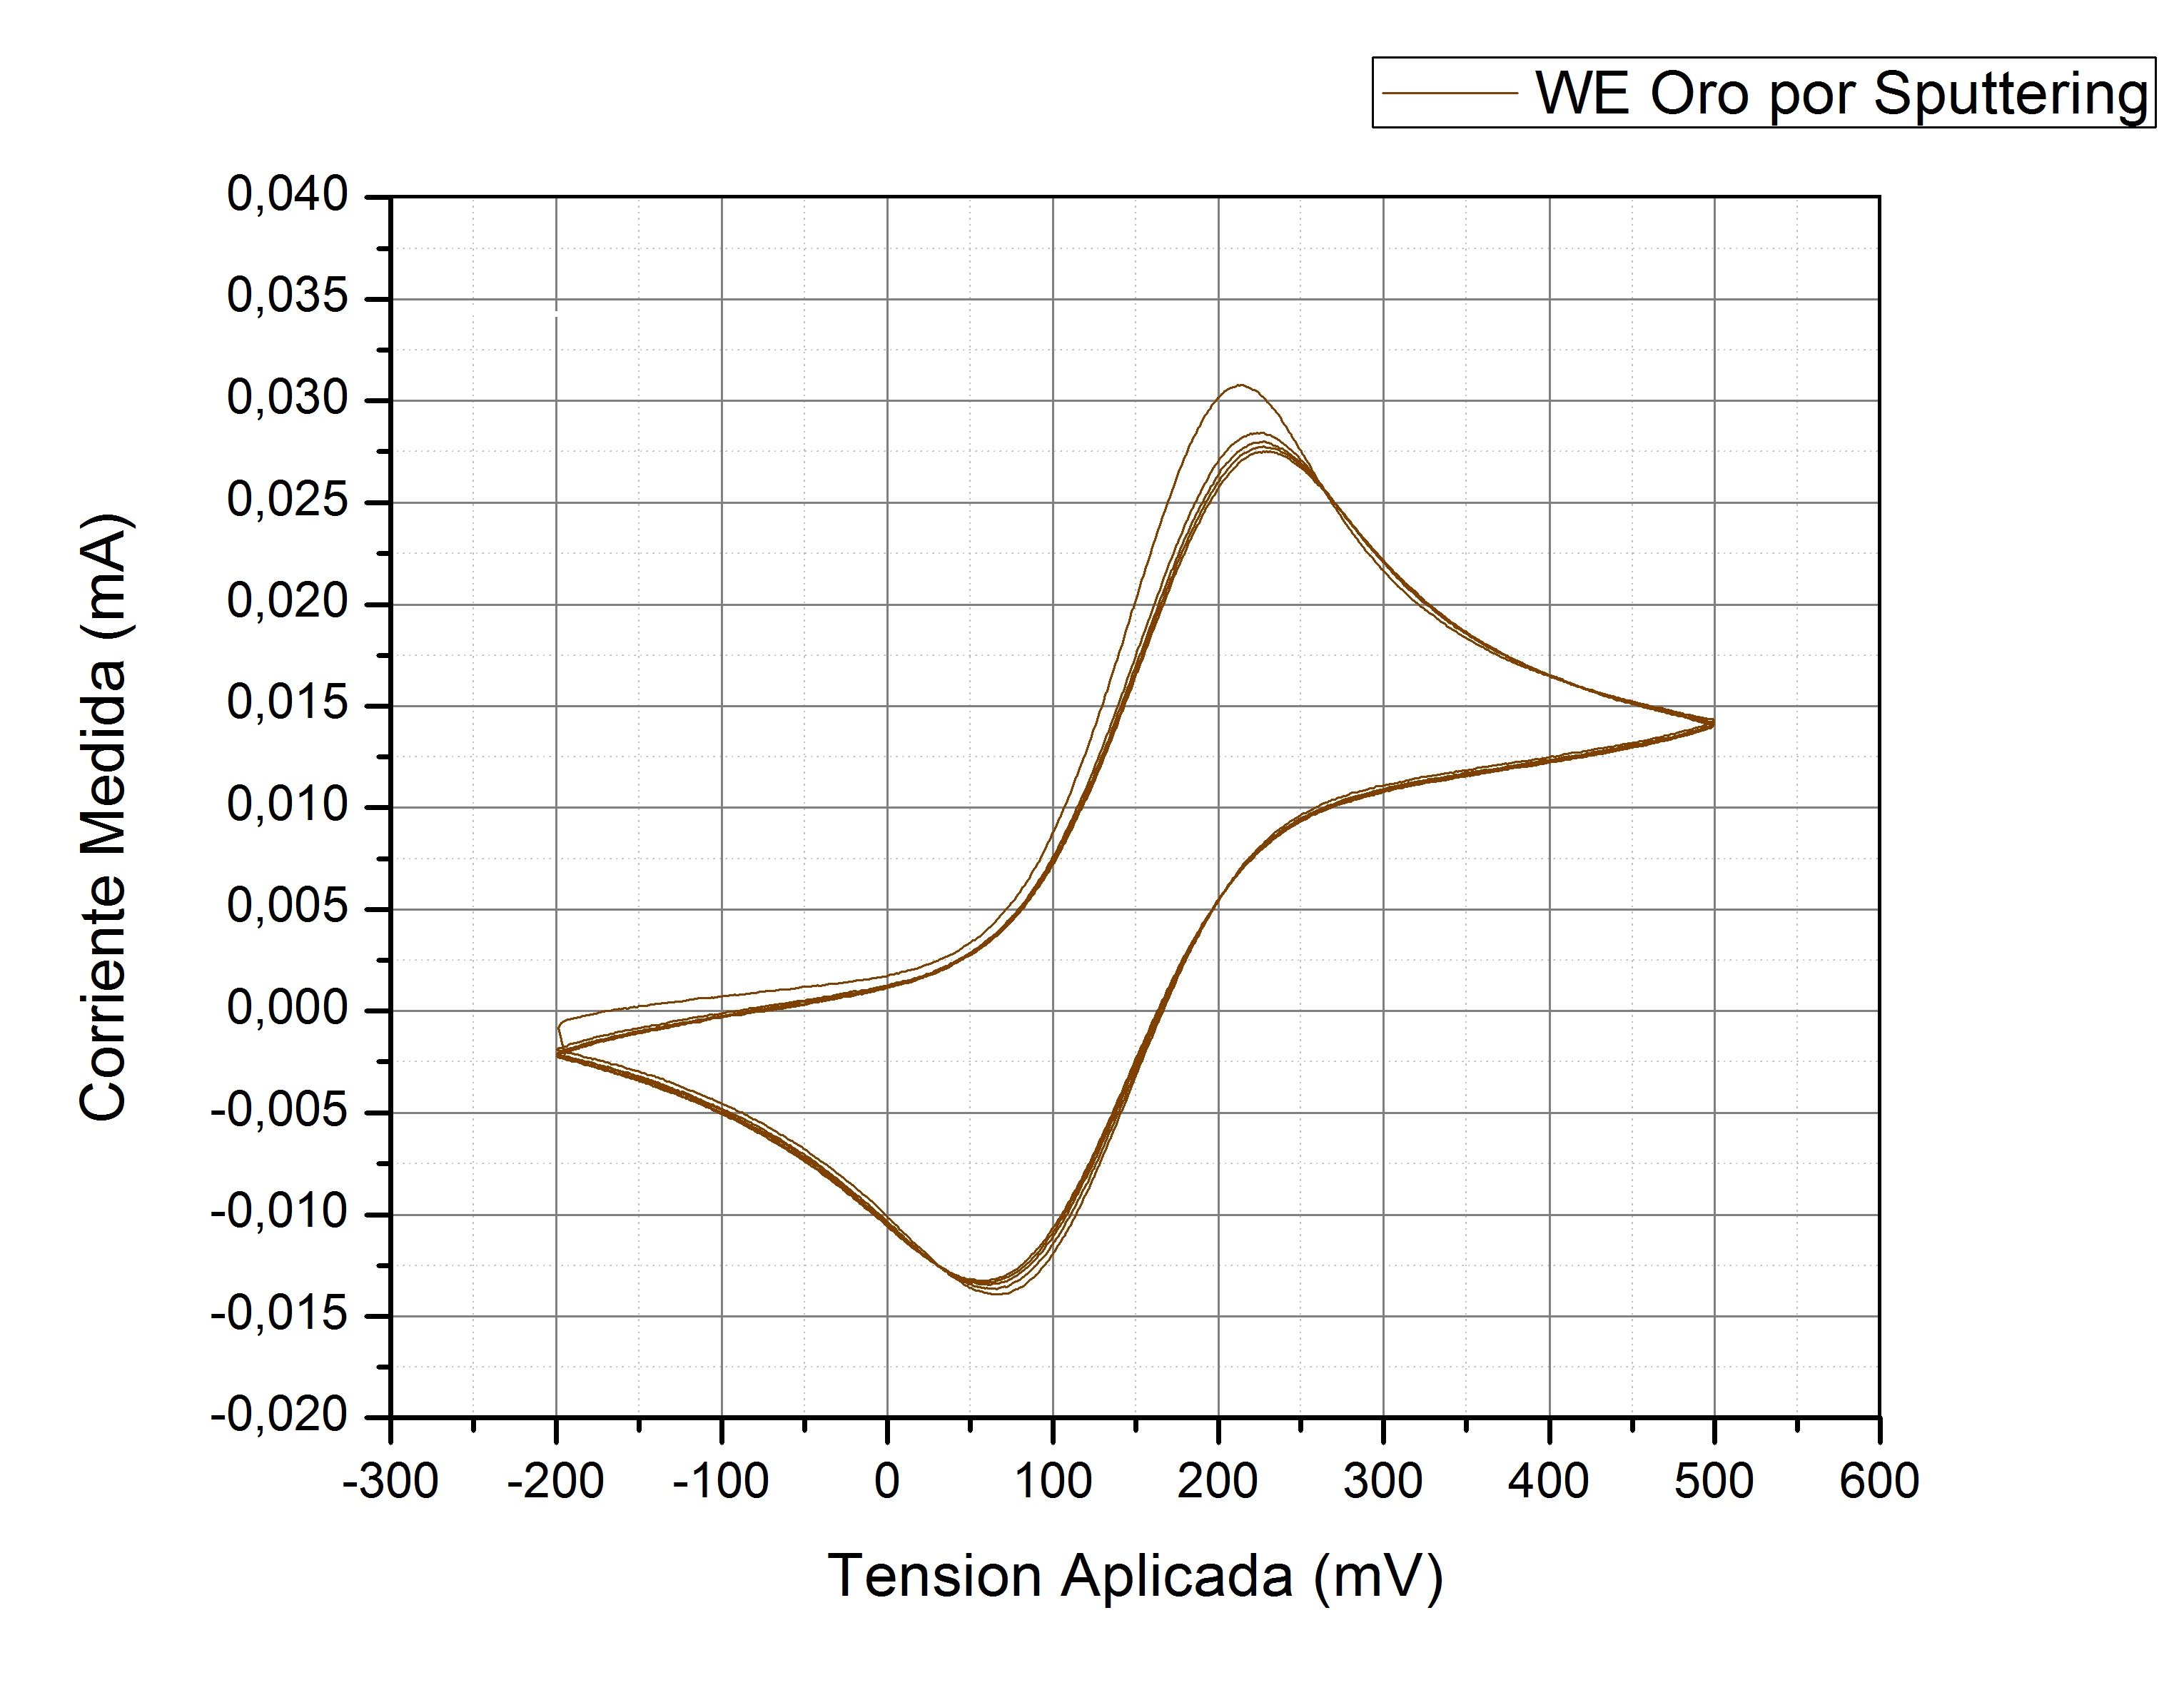
\includegraphics[width=0.8\textwidth]{Figuras/Figura_EQ_Oro_Sputtering_1mm}
  \caption{Voltametría cíclica con electrodo de oro obtenido por Sputtering.}
  \label{fig:Figura_EQ_Oro_Sputtering_1mm}
\end{figure}

Como segunda medición se optó por observar el comportamiento de las sondas electroquímicas sobre un electrodo de carbono (Figura ~\ref{fig:Figura_EQ_Carbono}), de esta forma se tienen las dos curvas que se superpondrían al probar un electrodo de carbono recubierto por la tinta de nanopartículas de oro.

\begin{figure}[H]
  \centering
    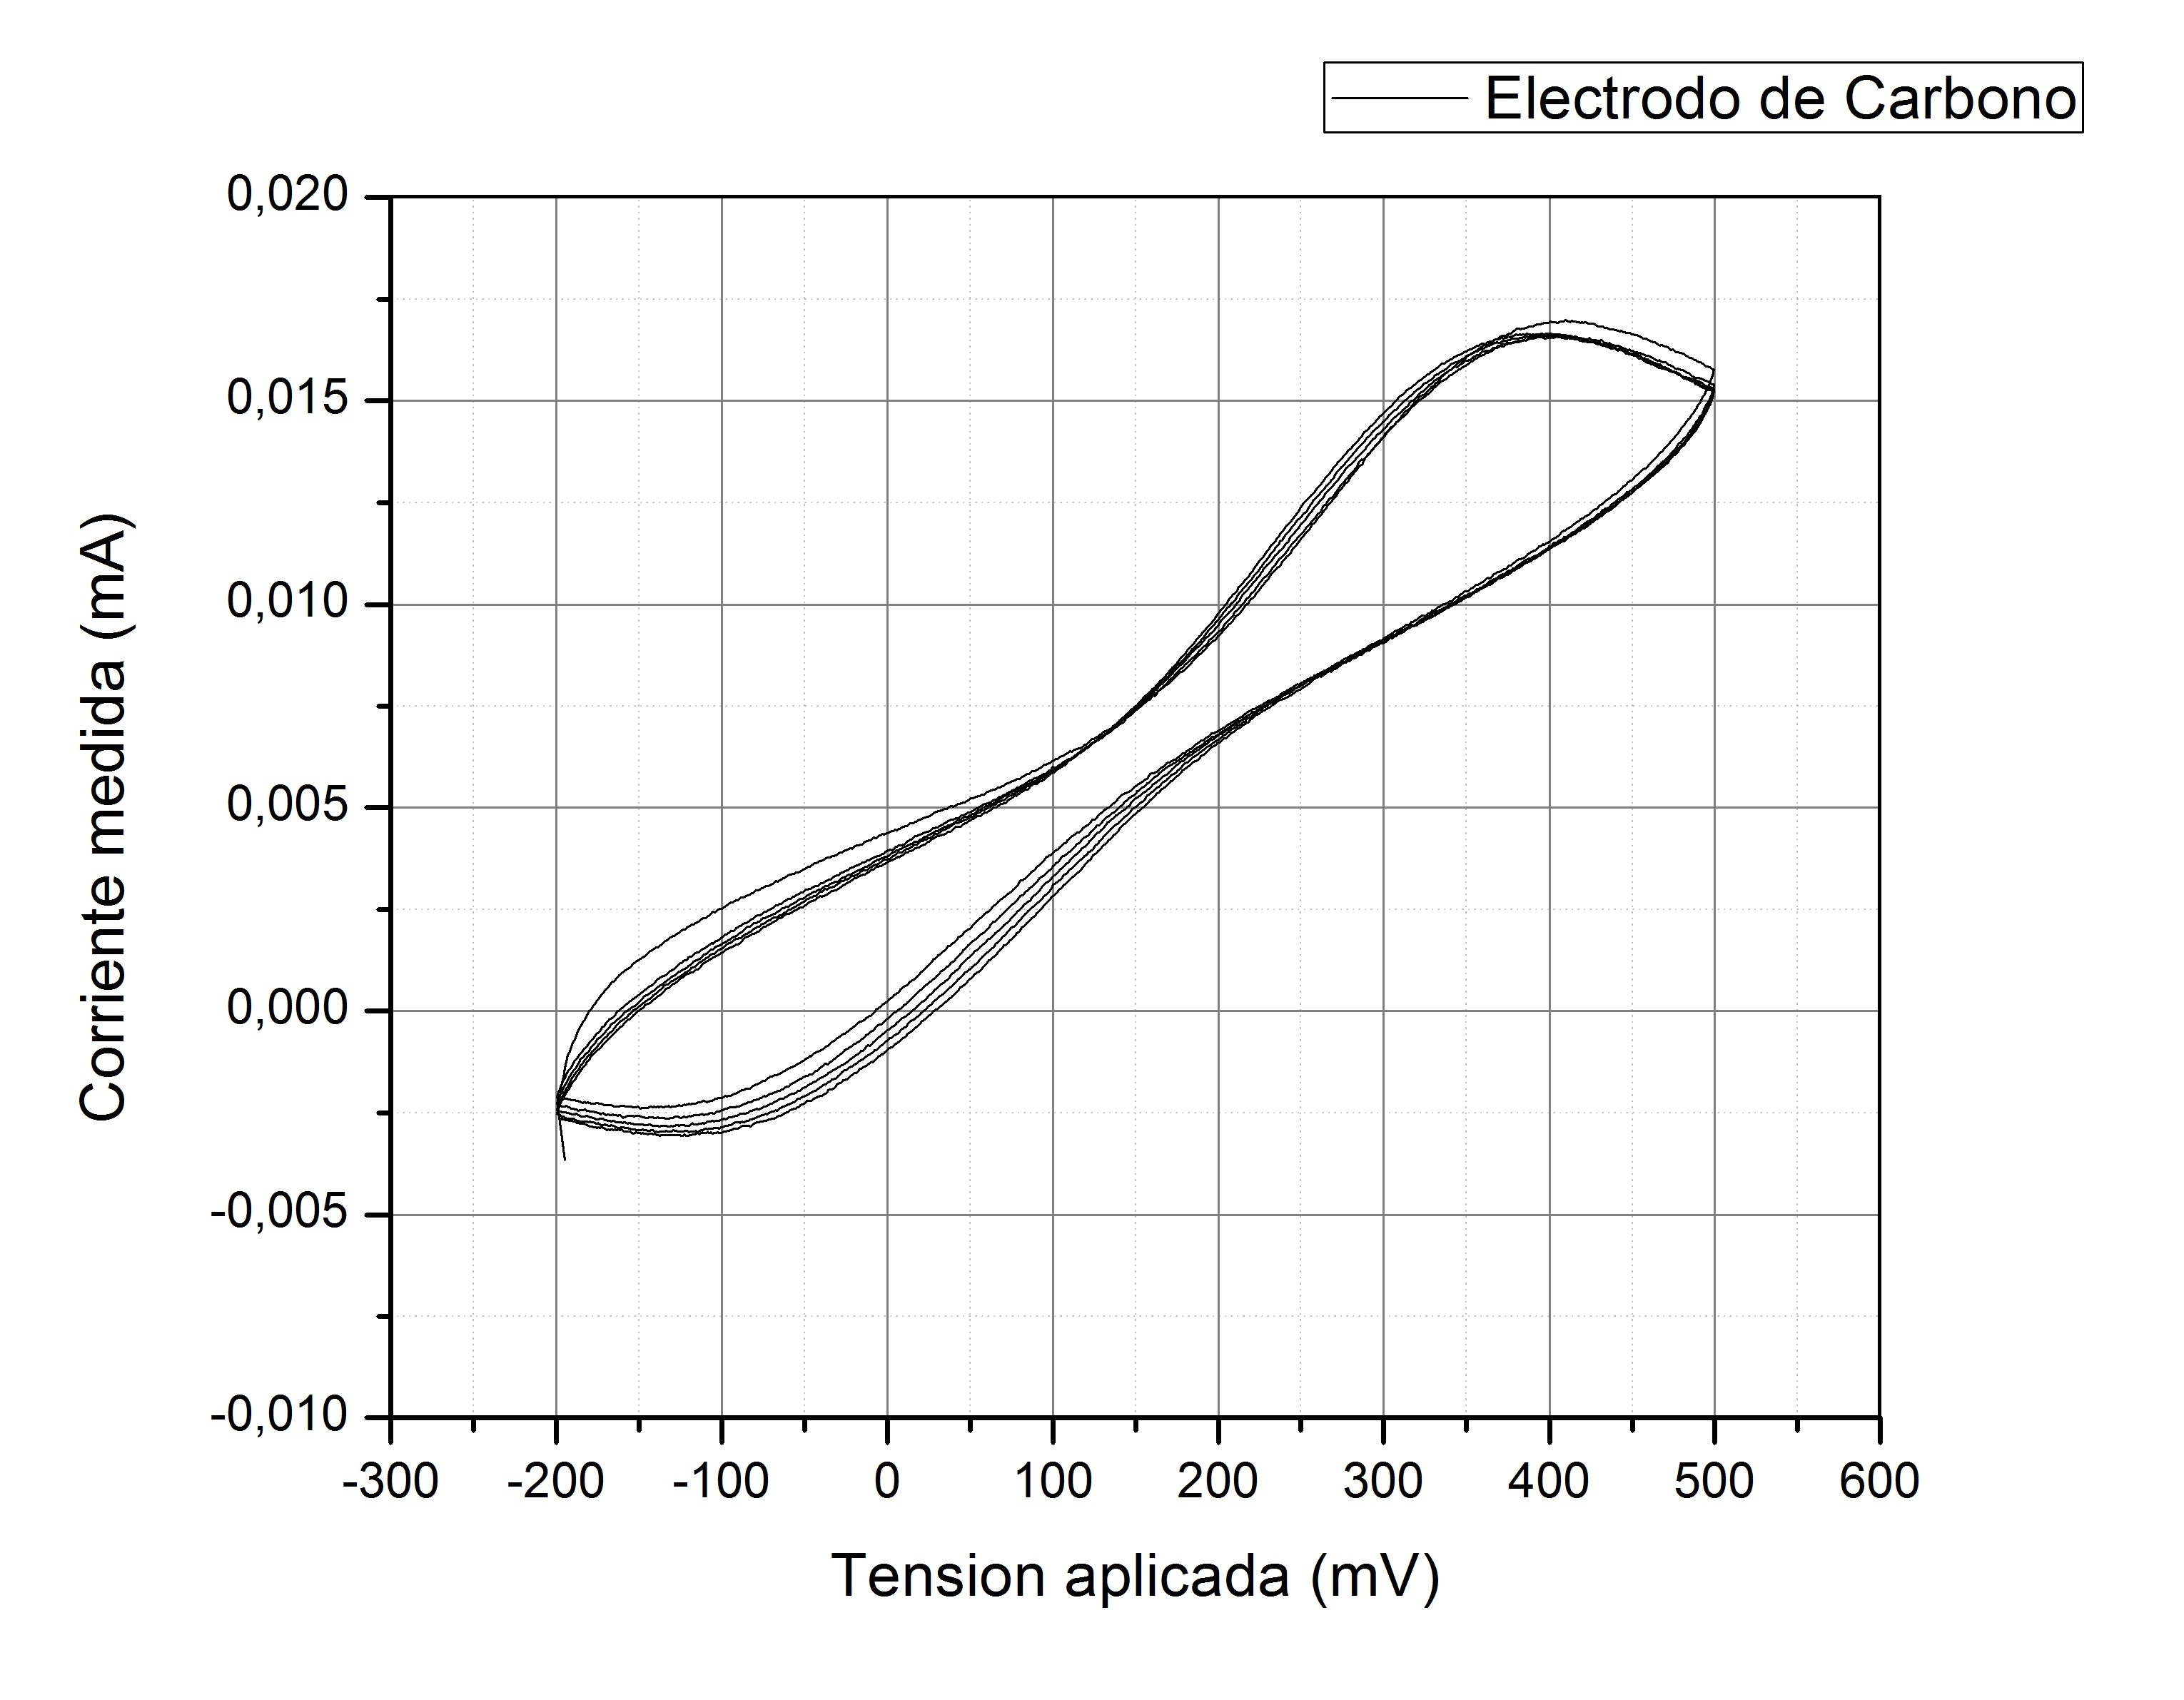
\includegraphics[width=0.8\textwidth]{Figuras/Figura_EQ_Carbono}
  \caption{Voltametría cíclica con electrodo de carbono.}
  \label{fig:Figura_EQ_Carbono}
\end{figure}
A continuación, se realizó la medición electroquímica sobre un electrodo de carbono recubierto con dos capas de tinta de nanopartículas de oro de 1 mm de diámetro (Figura ~\ref{fig:Figura_EQ_Oro_Inkjet_Ambos} (a)) y 1,1 mm de diámetro (Figura ~\ref{fig:Figura_EQ_Oro_Inkjet_Ambos} (b)).

Comparando el resultado de la curva voltamétrica cíclica de la celda electroquímica con \emph{WE} de oro depositado por \textit{Sputtering} con los \emph{WE} con tinta de nanopartículas de oro (Figura ~\ref{fig:Figura_EQ_Sputt_2-Inkjet}), se observa la similitud manteniéndose los picos de corriente correspondientes al oro.

\begin{figure}[H]
  \centering
    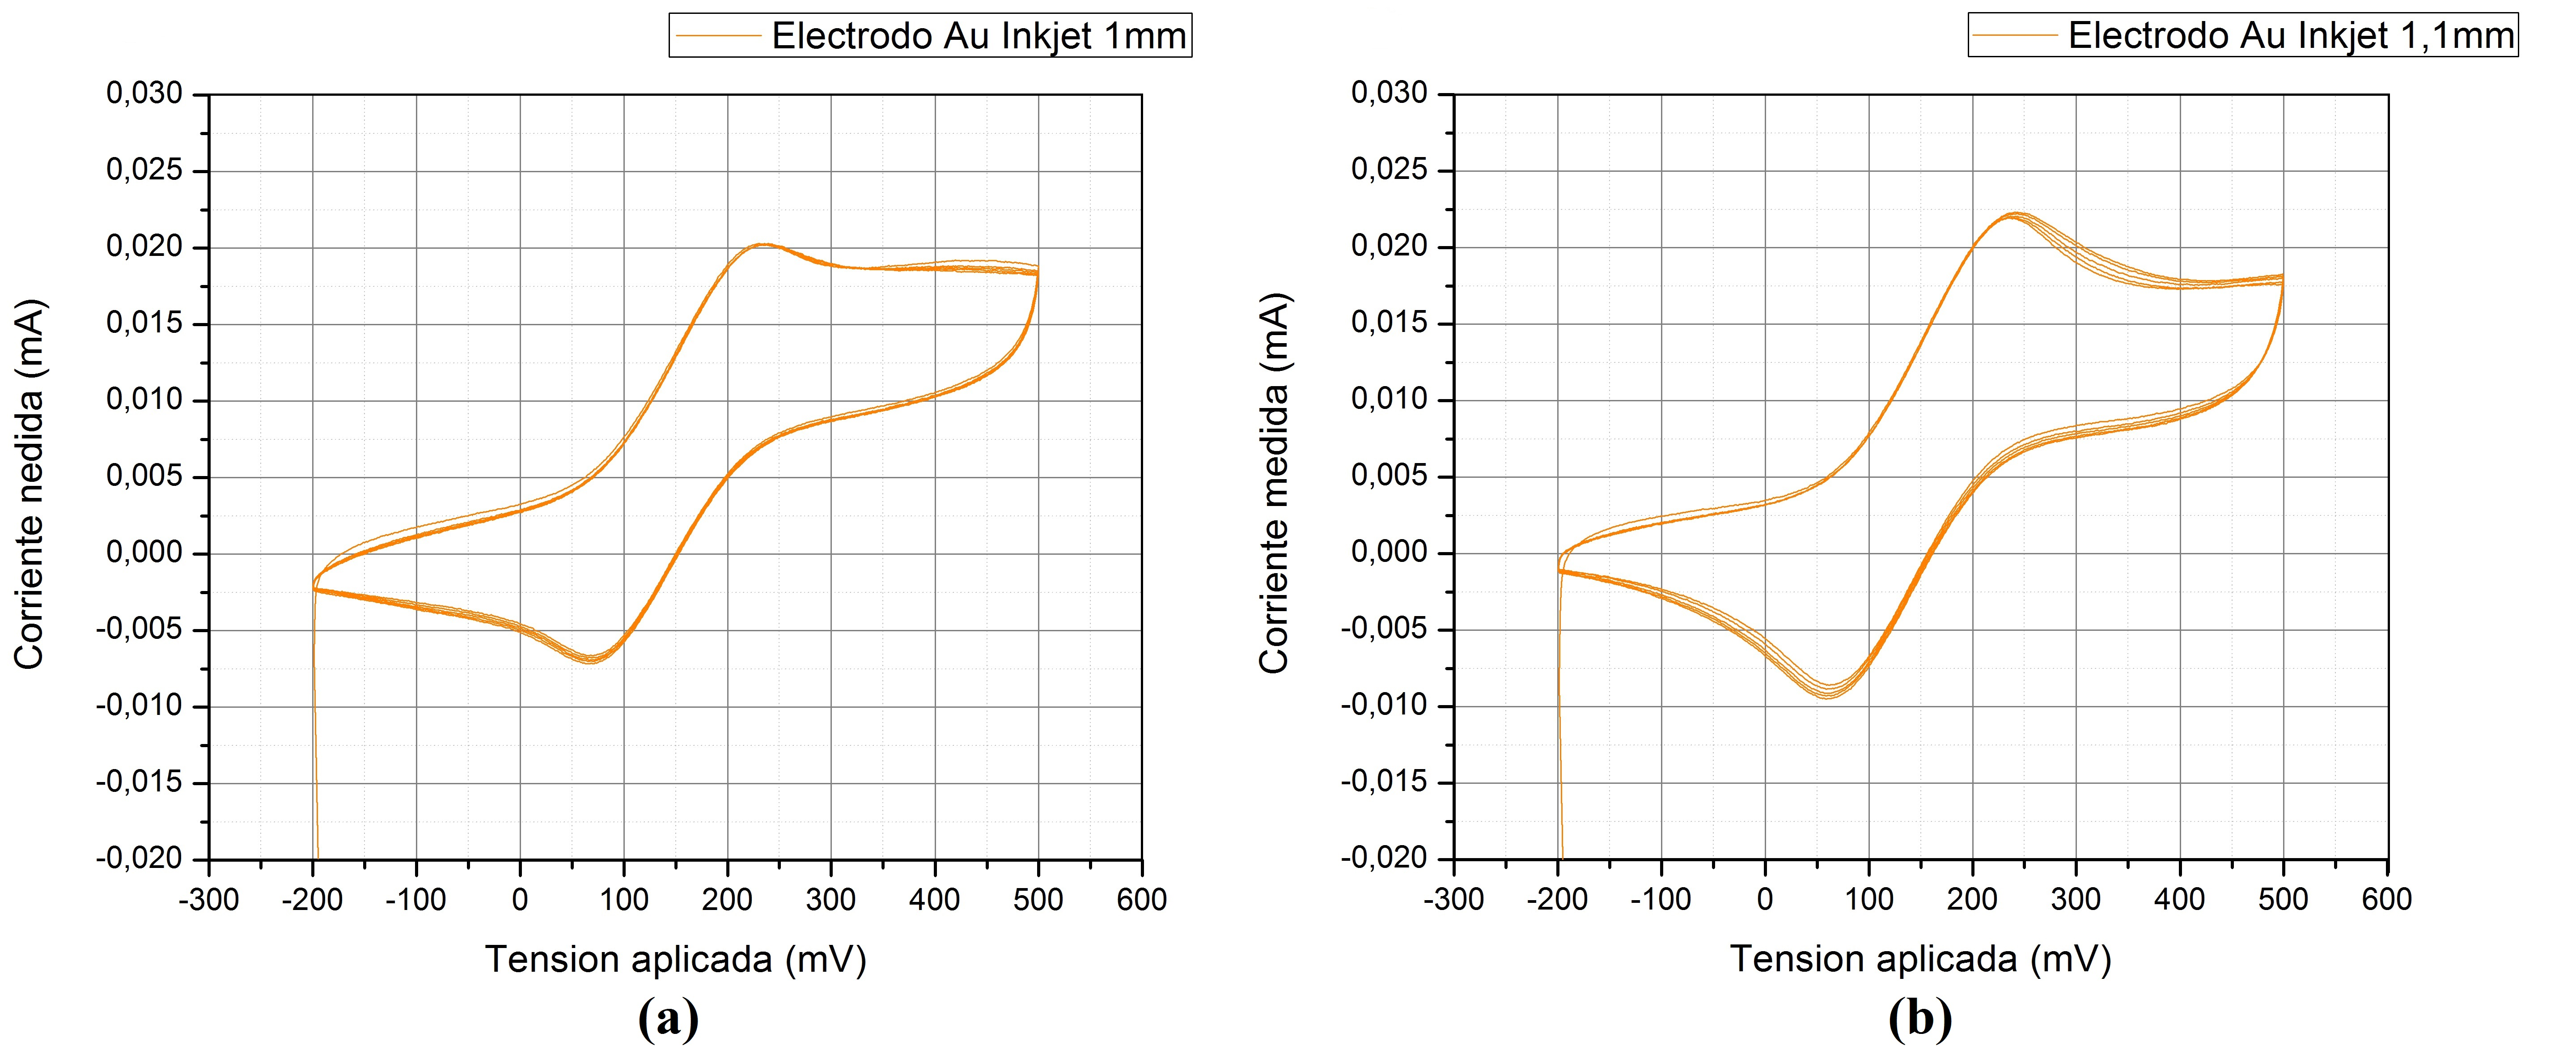
\includegraphics[width=1\textwidth]{Figuras/Figura_EQ_Oro_Inkjet_Ambos}
  \caption{Voltametría cíclica con \emph{WE} de carbono recubierto por tinta de nanopartículas de oro de diferentes diámetros: (a)1 mm; (b)1,1 mm.}
  \label{fig:Figura_EQ_Oro_Inkjet_Ambos}
\end{figure}

\begin{figure}[H]
  \centering
    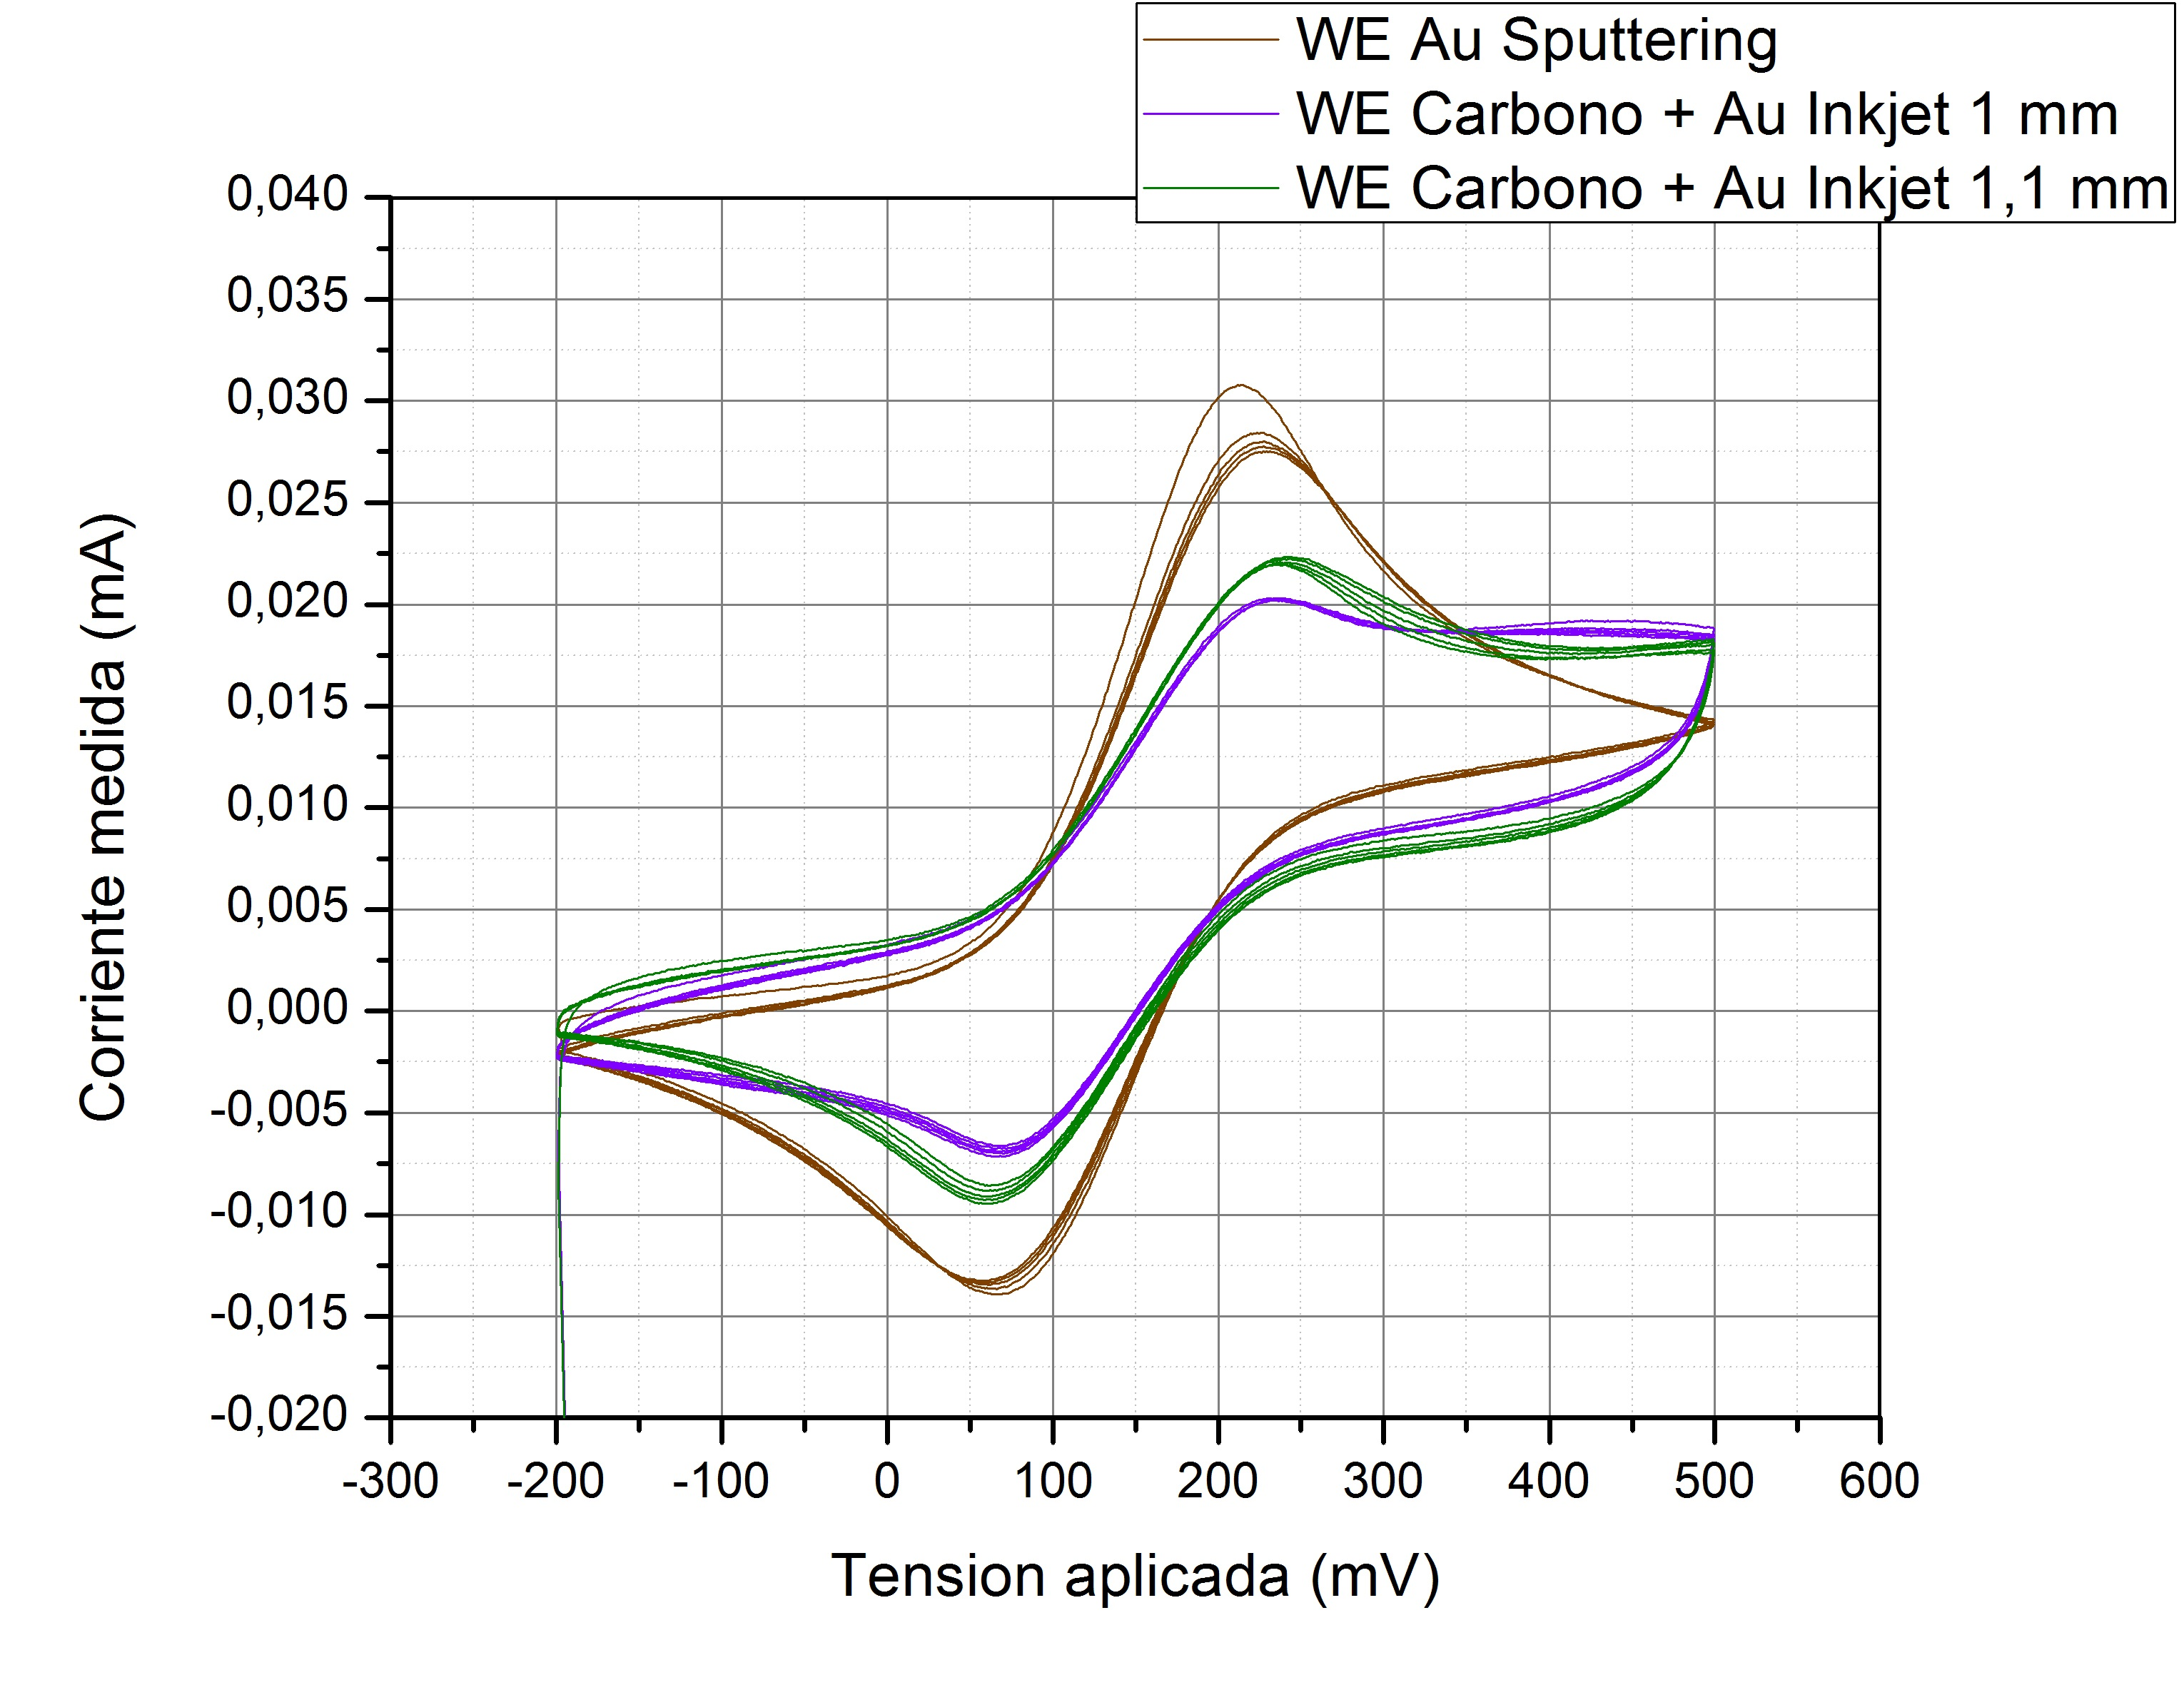
\includegraphics[width=0.8\textwidth]{Figuras/Figura_EQ_Sputt_2-Inkjet}
  \caption{Comparación de voltametrías cíclicas de celdas electroquímicas con \emph{WE} de oro depositado por \textit{Sputtering} y con \emph{WE} de carbono con tinta de nanopartículas de oro.}
  \label{fig:Figura_EQ_Sputt_2-Inkjet}
\end{figure}

El aumento de intensidad en los electrodos con impresión \textit{inkjet} de oro se debe a la presencia de carbono debajo de la misma, como se puede comprobar superponiendo las curvas anteriores con la del carbono puro (Figura ~\ref{fig:Figura_EQ_Oro_Inkjet_Ambos}) y además, al aumento del área efectiva de los \emph{WE} debido a la diferencia de rugosidad entre el oro depositado por \textit{sputtering} y la tinta de nanopartículas de oro impreso mediante \textit{inkjet}.

\begin{figure}[H]
  \centering
    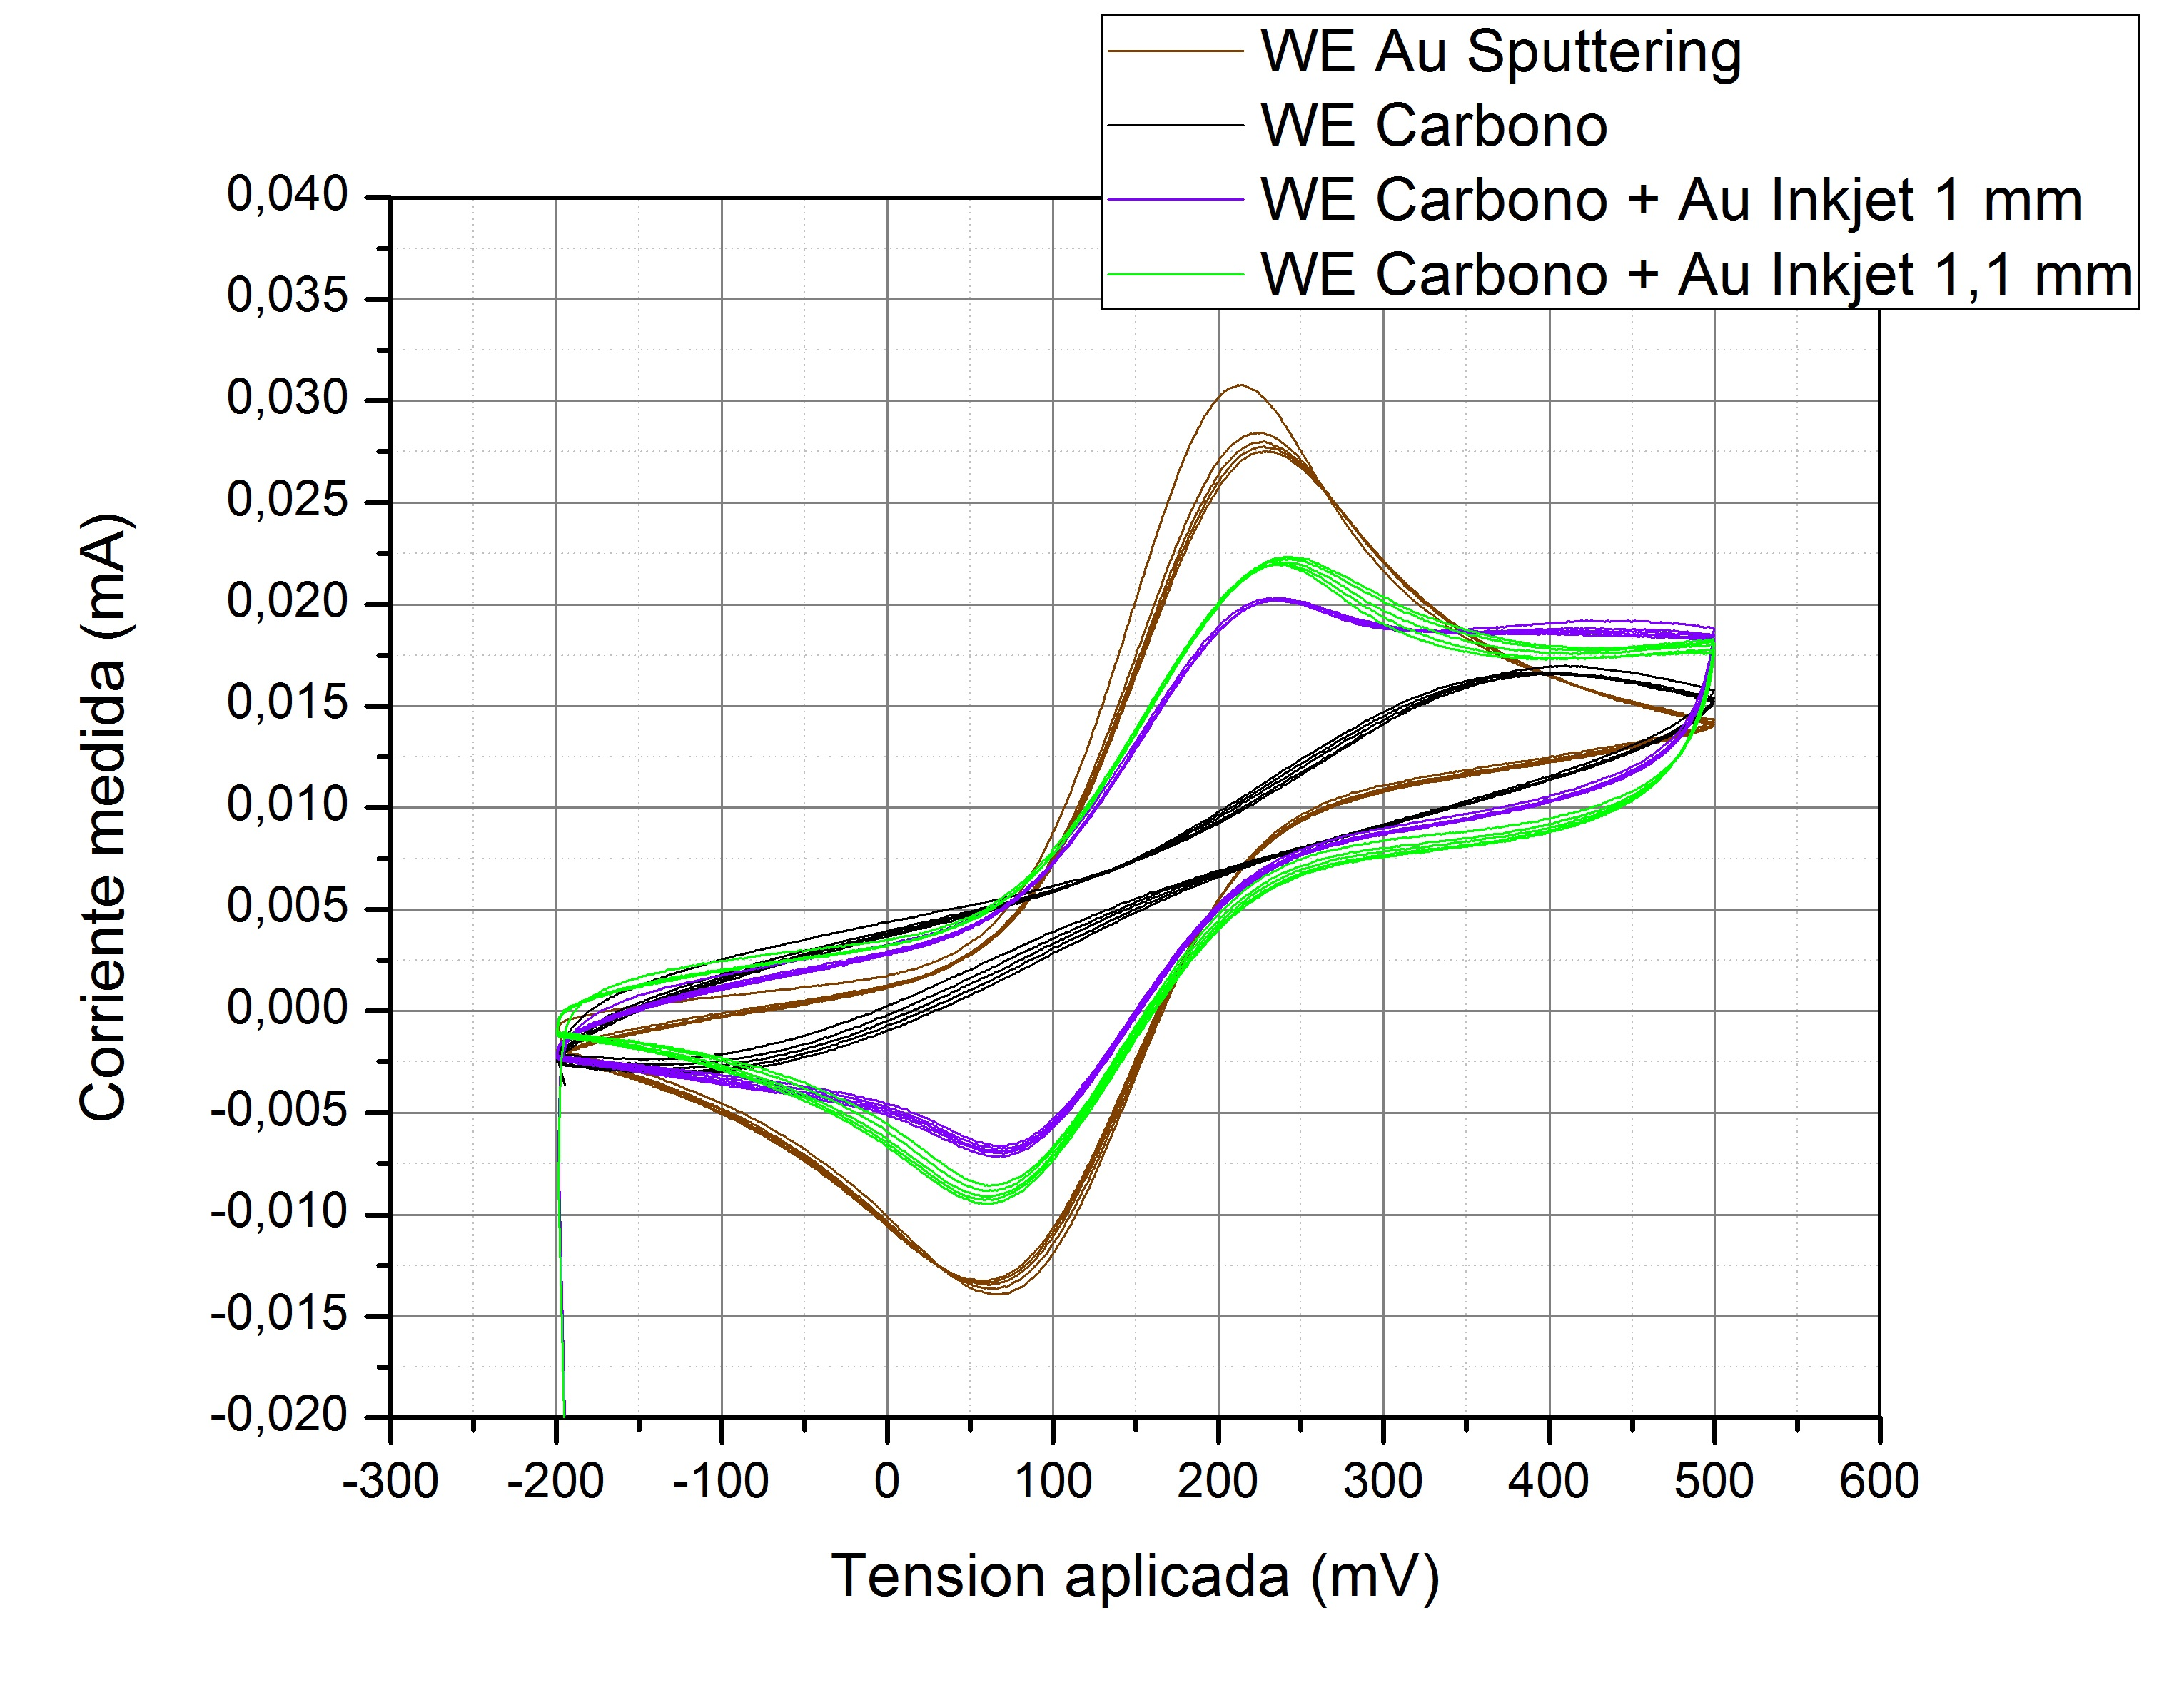
\includegraphics[width=0.8\textwidth]{Figuras/Figura_EQ_Sptt_AuInkjet_Carbono_Valox}
  \caption{Superposición de \emph{WE} con oro depositado por \textit{Sputtering}, \emph{WE} de carbono y \emph{WE} de carbono con tinta de nanopartículas de oro.}
  \label{fig:Figura_EQ_Sptt_AuInkjet_Carbono_Valox}
\end{figure}

Para tener comparaciones sobre la tinta de nanopartículas en diferentes sustratos, se realizaron mediciones de impresiones \textit{Inkjet} de la tinta sobre Valox, PET y hoja de pulpa de celulosa (Figura ~\ref{fig:Figura_EQ_Inkjet_Valox_PET_Papel}).

\begin{figure}[H]
  \centering
    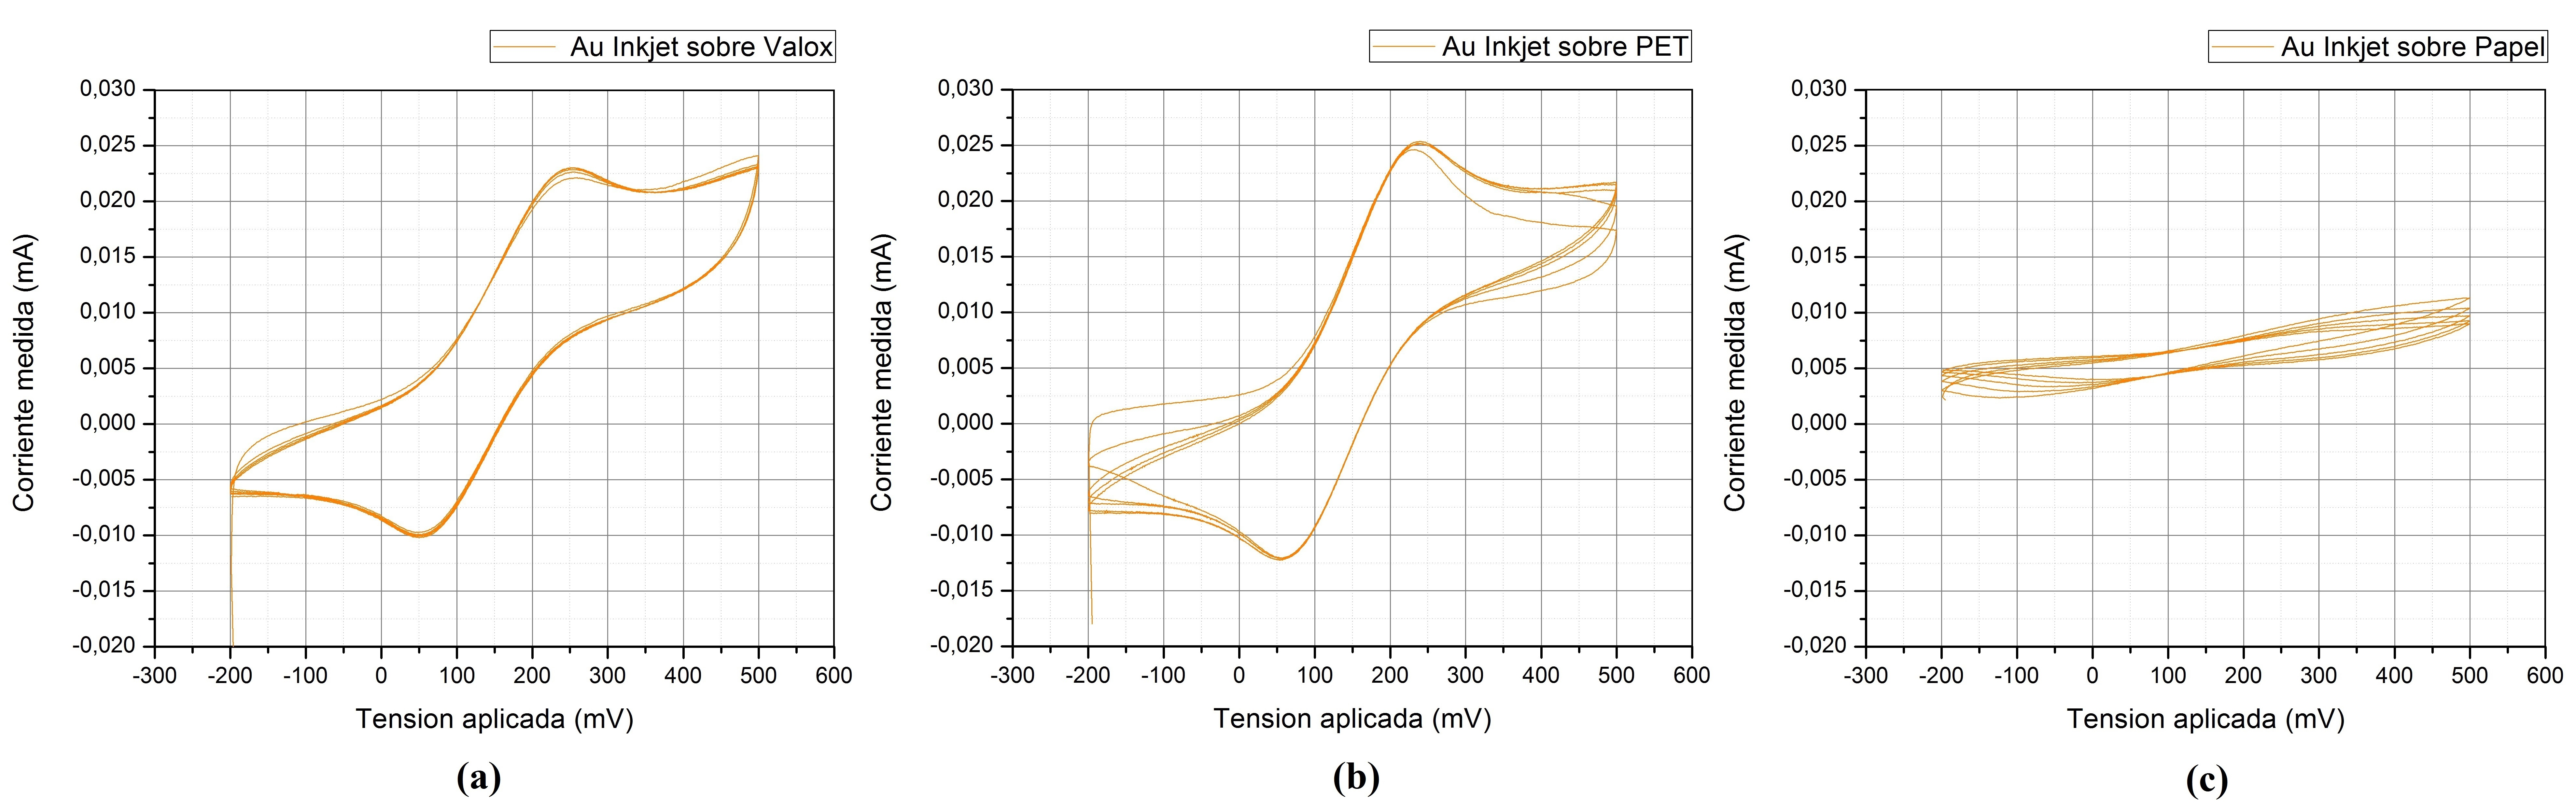
\includegraphics[width=1\textwidth]{Figuras/Figura_EQ_Inkjet_Valox_PET_Papel}
  \caption{Resultados de voltametría cíclica sobre impresión \textit{inkjet} de tinta con nanopartículas de oro sobre: (a)Valox; (b)PET y (c)Papel.}
  \label{fig:Figura_EQ_Inkjet_Valox_PET_Papel}
\end{figure}

Se destacan los resultados comparables obtenidos entre el oro depositado por \textit{Sputtering} y la impresión \textit{Inkjet} sobre sustrato liso (PET) (Figura ~\ref{fig:Figura_EQ_Sputt_Inkjet_PET}).

\begin{figure}[H]
  \centering
    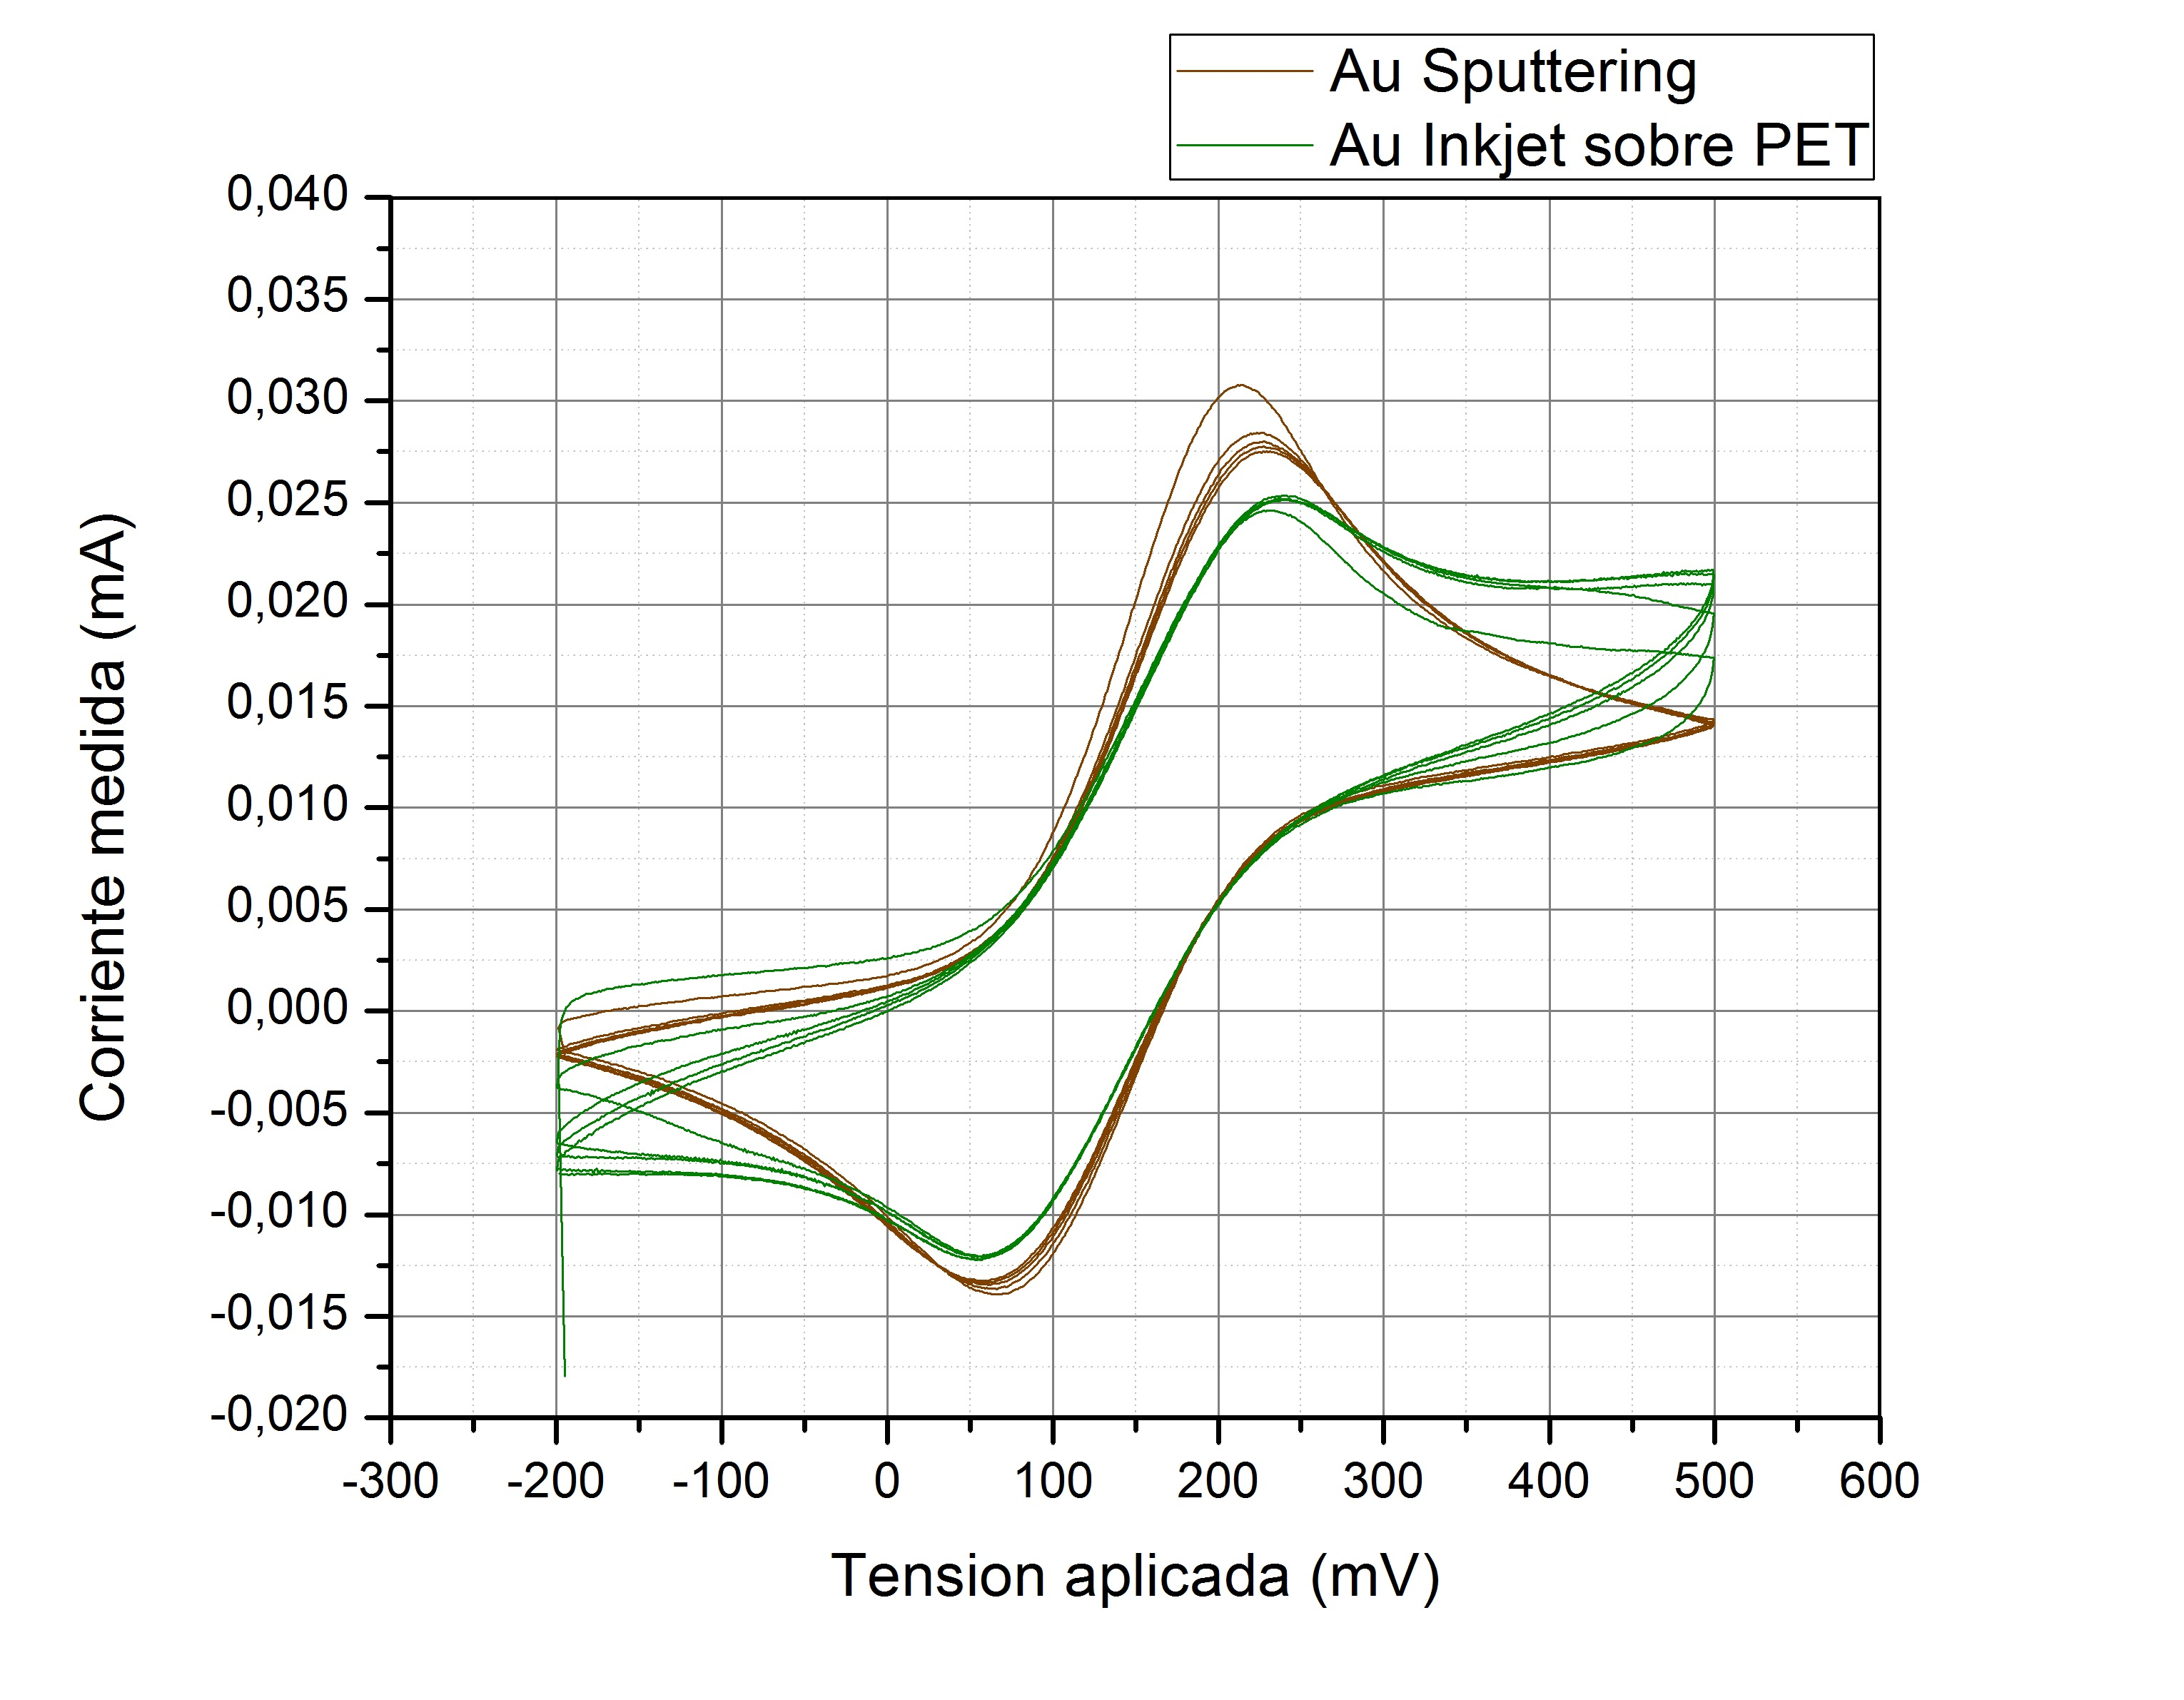
\includegraphics[width=0.8\textwidth]{Figuras/Figura_EQ_Sputt_Inkjet_PET}
  \caption{Comparación de voltametría cíclica sobre \emph{WE} de oro depositado por \textit{Sputtering} e impresión \textit{inkjet} de tinta con nanopartículas de oro sobre PET}
  \label{fig:Figura_EQ_Sputt_Inkjet_PET}
\end{figure}